\documentclass[10pt,a4paper]{article}

\usepackage[utf8]{inputenc}
\usepackage[T1]{fontenc}
\usepackage{lmodern}
\usepackage{microtype}
\usepackage[top=0.55in, bottom=0.5in, left=0.52in, right=0.52in]{geometry}
\usepackage{amsmath,amssymb}
\usepackage{booktabs}
\usepackage{array}
\usepackage{enumitem}
\usepackage{xcolor}
\usepackage{fancyhdr}
\usepackage{titlesec}
\usepackage{graphicx}
\usepackage{hyperref}

\DeclareUnicodeCharacter{2500}{\rule[0.5ex]{0.5em}{0.6pt}}

% Clean executive color palette
\definecolor{primaryblue}{RGB}{20, 56, 110}
\definecolor{accentblue}{RGB}{43, 92, 165}
\definecolor{successgreen}{RGB}{22, 115, 70}
\definecolor{warnorange}{RGB}{195, 90, 15}
\definecolor{dangerred}{RGB}{175, 35, 35}
\definecolor{codebg}{RGB}{244, 247, 251}
\definecolor{greenbg}{RGB}{240, 250, 244}
\definecolor{warnbg}{RGB}{254, 247, 238}
\definecolor{rulecolor}{RGB}{205, 214, 224}

\hypersetup{
    colorlinks=true,
    linkcolor=primaryblue,
    citecolor=primaryblue,
    urlcolor=accentblue,
    pdftitle={HIGH PERFORMANCE COMPUTING (BCSE414L) - Skew-Aware Adaptive Parallel Near-Duplicate Detection},
    pdfauthor={Lakshmi Sarupa Venkadesh (23BCE0463)}
}

\setlength{\parindent}{0pt}
\setlength{\parskip}{0.32em}
\emergencystretch=3em
\renewcommand{\_}{\textunderscore\allowbreak}
\setlist[itemize]{topsep=0.12em, itemsep=0.15em, leftmargin=1.3em}
\setlist[enumerate]{topsep=0.12em, itemsep=0.18em, leftmargin=1.4em}

% Ragged-right column types for clean tables
\newcolumntype{L}[1]{>{\raggedright\arraybackslash}p{#1}}
\newcolumntype{B}[1]{>{\raggedright\arraybackslash\bfseries}p{#1}}

% Section formatting
\titleformat{\section}
  {\normalfont\large\bfseries\color{primaryblue}}
  {}{0em}{}[\vspace{1.5pt}{\color{accentblue}\titlerule[0.8pt]}]
\titlespacing*{\section}{0pt}{0.65em}{0.3em}

\titleformat{\subsection}
  {\normalfont\normalsize\bfseries\color{accentblue}}
  {}{0em}{}
\titlespacing*{\subsection}{0pt}{0.45em}{0.18em}

% Header and Footer
\pagestyle{fancy}
\fancyhf{}
\fancyhead[L]{\footnotesize\bfseries\color{primaryblue}HIGH PERFORMANCE COMPUTING (BCSE414L) --- Project Review}
\fancyhead[R]{\footnotesize\color{black!70}Group 29 --- Lakshmi Sarupa Venkadesh (\texttt{23BCE0463})}
\fancyfoot[C]{\footnotesize\color{black!65}Page \thepage\ of 3}
\renewcommand{\headrulewidth}{0.4pt}
\renewcommand{\footrulewidth}{0pt}

% Helper macro for KPI stat cards
\newcommand{\statcard}[3]{%
    \fcolorbox{accentblue}{codebg}{%
        \parbox[t][1.52cm][c]{0.226\textwidth}{%
            \centering
            {\Large\bfseries\color{#1}#2}\\[2pt]
            {\scriptsize\bfseries\color{black!80}#3}
        }%
    }%
}

\begin{document}
\sloppy

% ============================================================================
% PAGE 1: OVERVIEW, KPI CARDS, DEFINITIONS & EXISTING VS. PROPOSED
% ============================================================================
\begin{center}
    \fcolorbox{primaryblue}{codebg}{%
        \parbox{0.98\textwidth}{%
            \vspace{0.14cm}
            \centering
            {\scriptsize\bfseries\color{accentblue}SCHOOL OF COMPUTER SCIENCE AND ENGINEERING $\bullet$ HIGH PERFORMANCE COMPUTING (BCSE414L) $\bullet$ GROUP 29}\\[0.1cm]
            {\LARGE\bfseries\color{primaryblue}Skew-Aware Adaptive Parallel Near-Duplicate Detection on Multicore CPUs}\\[0.08cm]
            {\footnotesize\color{black!80}\textbf{Lakshmi Sarupa Venkadesh (\texttt{23BCE0463})} $\quad|\quad$ Faculty Guide: Prof.\ Vimala Devi K. $\quad|\quad$ C++17 \& OpenMP}
            \vspace{0.14cm}
        }%
    }
\end{center}

\vspace{0.02cm}

\begin{center}
    \statcard{successgreen}{4.41$\times$ Speedup}{End-to-End at $N=8000$ Skewed ($656.1\text{ ms} \to 148.7\text{ ms}$)}\hfill
    \statcard{primaryblue}{68.35\% Filtered}{Redundant Multi-Band Pairs Suppressed in Registers}\hfill
    \statcard{warnorange}{90.16\% Skew}{Of All $8.62\text{M}$ Pairs Concentrated in 17 Heavy Buckets}\hfill
    \statcard{successgreen}{100\% Parity}{Bitwise-Identical Output Across 3,400 Measured Runs}
\end{center}

\vspace{0.02cm}

\fcolorbox{successgreen}{greenbg}{%
    \parbox{0.98\textwidth}{\footnotesize
        \textbf{\color{successgreen}Executive Summary:}
        \begin{itemize}[leftmargin=1.3em, topsep=0.08em, itemsep=0.1em]
            \item \textbf{Problem Statement:} SimHash band indexing avoids $\mathcal{O}(N^2)$ all-pairs checks by hashing documents into candidate buckets. However, skewed real-world text clusters produce oversized buckets whose pairwise work grows quadratically as $W_b = \frac{k(k-1)}{2}$ ($>1.17\text{M}$ pairs in one bucket).
            \item \textbf{Limitation of Standard OpenMP:} Built-in loop policies (\texttt{static}, \texttt{dynamic}, \texttt{guided}) schedule whole buckets as atomic iterations, trapping individual threads on oversized buckets while other cores idle.
            \item \textbf{Proposed Architecture:} Our pipeline pre-computes exact bucket costs $\frac{k(k-1)}{2}$ and Coefficient of Variation ($\text{CV}$), decomposes oversized buckets ($W_b > 4\overline{W}$) into bounded \textbf{4,096-pair chunks} via $\mathcal{O}(\log k)$ triangular unranking, merges candidates in parallel across 64 ID-range partitions, and suppresses $68.35\%$ of redundant multi-band emissions in CPU registers via a branch-free 64-bit SWAR zero-byte check.
        \end{itemize}
    }%
}

\section{1. Core Concepts, Metrics \& Pipeline Architecture}

\begingroup
\footnotesize
\renewcommand{\arraystretch}{1.18}
\begin{tabular}{@{} >{\raggedright\arraybackslash\bfseries\color{primaryblue}}p{0.24\textwidth} L{0.73\textwidth} @{}}
    \toprule
    \textbf{Concept / Metric} & \textbf{Technical Definition} \\
    \midrule
    3-Word Shingling \& SimHash & Overlapping 3-word tokens are hashed via deterministic 64-bit FNV-1a and aggregated by weighted bit voting into a 64-bit SimHash fingerprint; near-duplicates satisfy Hamming distance $d_H(\text{fp}_u, \text{fp}_v) = \text{popcount}(\text{fp}_u \oplus \text{fp}_v) \le 3$. \\
    8-Band Pigeonhole Indexing & Each 64-bit fingerprint is partitioned into \textbf{8 disjoint 8-bit bands} ($8 \times 256 = 2,048$ buckets). By the Pigeonhole Principle, any pair with $d_H \le 7$ shares at least one identical band ($100\%$ algorithmic candidate recall for $d_H \le 3$). \\
    Quadratic Bucket Cost ($W_b$) & A bucket with $k$ documents requires $W_b = \frac{k(k-1)}{2}$ pairwise evaluations ($k=10 \to 45$ pairs; $k=1,534 \to \mathbf{1,175,811}$ pairs). \\
    Bucket Skew ($\text{CV}$) \& Imbalance ($I$) & $\text{CV} = \sigma / \overline{W}$ measures bucket work dispersion ($\text{CV} = 0.60$ Balanced vs.\ $\mathbf{13.55}$ Skewed at $N=8,000$). Thread Work Imbalance $I = \frac{\max_t(W_t)}{\text{mean}_t(W_t)}$ measures load balance across active threads ($I = 1.00$ is ideal). \\
    SWAR Band Suppression & Branch-free 64-bit bitwise zero-byte test on $\text{fp}_u \oplus \text{fp}_v$ that detects in $\mathcal{O}(1)$ whether a candidate pair already collided in any earlier band $0 \dots b-1$, preventing duplicate candidate buffer writes at emission time. \\
    \bottomrule
\end{tabular}
\endgroup

\vspace{0.2em}
\begin{center}
\fcolorbox{rulecolor}{codebg}{%
\parbox{0.98\textwidth}{\centering\scriptsize\bfseries\color{primaryblue}
[Stage 1: Parallel 64-bit SimHash] $\longrightarrow$
[Stage 2: $8\times 8$-bit Band Buckets + $\text{CV}$ Stats] $\longrightarrow$
[Stage 3a--d: Heavy-Bucket Chunk Split (4,096 pairs) + SWAR Filter] $\longrightarrow$
[Stage 3e: Parallel 64-Partition Sort/Dedup] $\longrightarrow$
[Stage 4: Parallel POPCNT Verify ($d_H \le 3$)]
}}
\end{center}

\section{2. Existing Approaches vs.\ Proposed Skew-Aware Architecture}

\begingroup
\footnotesize
\renewcommand{\arraystretch}{1.20}
\begin{tabular}{@{} B{0.23\textwidth} L{0.36\textwidth} L{0.36\textwidth} @{}}
    \toprule
    \textcolor{primaryblue}{Method / Paradigm} & \textcolor{dangerred}{\textbf{Mechanism \& Limitation Under Skew}} & \textcolor{successgreen}{\textbf{Proposed Skew-Aware Solution}} \\
    \midrule
    1. Heuristic Bucket Truncation & Drops or sub-samples buckets exceeding a fixed size cap $K$. \textbf{Limitation:} Sacrifices recall (\textbf{False Negatives}). & \textbf{Exact Evaluation:} Processes $100\%$ of pairs with $100\%$ recall ($d_H \le 7$) and exact bitwise output parity. \\
    2. Distributed Key Salting (Spark / MapReduce) & Appends random suffixes to hot keys to split reducers across nodes. \textbf{Limitation:} High network shuffle and RAM overhead. & \textbf{Shared-Memory Efficiency:} Executes in-place on multicore CPU vectors with $<0.09\text{ ms}$ scheduling overhead. \\
    3. Fixed OpenMP Loops (\texttt{static / dynamic / guided}) & Schedules 1 whole bucket per loop iteration. \textbf{Limitation:} Straggler thread on heavy buckets; \texttt{dynamic} causes Stage 4 queue contention ($438.8\text{ ms}$). & \textbf{Intra-Bucket Chunking:} Decomposes oversized buckets ($W_b > 4\overline{W}$) into \textbf{4,096-pair tasks} shared across all threads. \\
    4. Runtime Work-Stealing Schedulers & Reacts post-hoc via runtime queues; cannot subdivide a single loop iteration. & \textbf{Analytical Pre-Costing:} Uses exact $\frac{k(k-1)}{2}$ cost prior to execution with $\mathcal{O}(\log k)$ pair index unranking. \\
    \bottomrule
\end{tabular}
\endgroup

\newpage

% ============================================================================
% PAGE 2: BENCHMARK NUMBERS, OPTIMIZATION PROGRESSION & TECH STACK
% ============================================================================
\section{3. Experimental Benchmark Results ($N = 8,000$ Skewed, $T = 8$ Threads)}

\begin{itemize}[leftmargin=1.3em]
    \item \textbf{Workload Skew Profile ($N=8,000$, $\text{CV} = 13.55$):} Generates \textbf{8,615,757 pair evaluations} ($8.17\times$ higher than Balanced $1.05\text{M}$). Just \textbf{17 oversized buckets} out of 2,048 contain \textbf{7,767,834 pairs (90.16\% of total work)}, with $k_{\max} = 1,534$ documents (\textbf{1,175,811 pairs}).
    \item \textbf{Minimal Scheduling Overhead:} Bucket classification (\texttt{Stage 3a}: \textbf{0.024 ms}) and splitting the 17 heavy buckets into \textbf{1,904 chunks} (\texttt{Stage 3c}: \textbf{0.055 ms}) add less than \textbf{0.09 ms} combined.
\end{itemize}

\vspace{0.1em}
\fcolorbox{rulecolor}{white}{%
\parbox{0.98\textwidth}{%
\vspace{0.08cm}
\textbf{\footnotesize\color{primaryblue}Step-by-Step Optimization Progression at $N = 8,000$ Skewed ($T = 8$ Threads):}\\[0.12cm]
\footnotesize
\renewcommand{\arraystretch}{1.30}
\begin{tabular}{@{} L{0.45\textwidth} r r L{0.30\textwidth} @{}}
    \textbf{Pipeline Configuration / Optimization Phase} & \textbf{Median Time} & \textbf{Speedup} & \textbf{Relative Runtime (Lower = Faster)} \\
    \hline
    1. Sequential Baseline ($T=1$, Reference) & \texttt{656.05 ms} & \textbf{1.00$\times$} & \textcolor{dangerred}{\rule{4.5cm}{6.5pt}} \\
    2. OpenMP Dynamic ($T=8$, Stage 4 Queue Contention) & \texttt{684.68 ms} & \textbf{0.96$\times$} & \textcolor{dangerred}{\rule{4.7cm}{6.5pt}} \\
    3. Phase 8: Adaptive Bucket Split (Serial Stage 3e Merge) & \texttt{587.44 ms} & \textbf{1.09$\times$} & \textcolor{warnorange}{\rule{4.03cm}{6.5pt}} \\
    4. Phase 9: + Parallel 64-Partition Merge \& Dedup & \texttt{294.95 ms} & \textbf{2.22$\times$} & \textcolor{accentblue}{\rule{2.02cm}{6.5pt}} \\
    5. Phase 10: + SWAR Band Suppression ($T=8$) & \texttt{148.72 ms} & \textbf{4.41$\times$} & \textcolor{successgreen}{\rule{1.02cm}{6.5pt}} \\
\end{tabular}
\vspace{0.08cm}
}}

\subsection*{Cross-Policy Performance \& Stage Breakdown ($N = 8,000$ Skewed, 3,400 Measured Runs)}

\begingroup
\footnotesize
\setlength{\tabcolsep}{4.8pt}
\renewcommand{\arraystretch}{1.20}
\begin{tabular}{@{} L{0.35\textwidth} r r r r r @{}}
    \toprule
    \textbf{Measured Metric ($N = 8,000$ Skewed)} & \textbf{Seq ($1T$)} & \textbf{Dynamic ($8T$)} & \textbf{Guided ($8T$)} & \textbf{Adaptive ($8T$)} & \textbf{Adaptive+SWAR ($8T$)} \\
    \midrule
    \textbf{Total End-to-End Runtime (ms)} & 656.05 ms & 684.68 ms & 313.77 ms & 294.95 ms & \textbf{\color{successgreen}148.72 ms} \\
    \textbf{Total Speedup ($S_p = T_1 / T_p$)} & $1.00\times$ & $0.96\times$ & $2.09\times$ & $2.22\times$ & \textbf{\color{successgreen}4.41$\times$} \\
    \textbf{Stage 3 Candidate Gen Total (ms)} & 511.84 ms & 220.25 ms & 205.82 ms & 218.99 ms & \textbf{\color{successgreen}76.91 ms (-85\%)} \\
    \textbf{Stage 3d Heavy-Bucket Chunks (ms)} & --- & --- & --- & 53.56 ms & \textbf{\color{successgreen}15.11 ms} \\
    \textbf{Stage 3e Merge, Sort \& Dedup (ms)} & --- & --- & --- & 157.91 ms & \textbf{\color{successgreen}56.28 ms} \\
    \textbf{Stage 4 Hamming Verification (ms)} & 36.68 ms & \textcolor{dangerred}{\textbf{438.79 ms}} & 65.19 ms & 39.66 ms & \textbf{40.01 ms} \\
    \textbf{Work Imbalance ($I$ at $T=4$ / $T=8$)} & $1.000$ & $1.257 / 1.590$ & $1.131 / 1.719$ & \textbf{\color{successgreen}1.078} / $1.308$ & \textbf{\color{successgreen}1.078} / $1.308$ \\
    \textbf{Candidate Buffer Footprint (MB)} & 137.85 MB & 137.85 MB & 137.85 MB & 137.85 MB & \textbf{\color{successgreen}43.63 MB (-94.2 MB)} \\
    \textbf{Participating Threads / Parity} & 1/1 (PASS) & 8/8 (PASS) & 8/8 (PASS) & \textbf{8/8 (PASS)} & \textbf{8/8 (PASS)} \\
    \bottomrule
\end{tabular}
\endgroup

\section{4. System Architecture, Tech Stack \& Algorithmic Optimizations}

\begin{minipage}[t]{0.47\textwidth}
\raggedright
\subsection*{Hardware, Compiler \& Build Environment}
\footnotesize
\begin{itemize}[leftmargin=1.2em]
    \item \textbf{Processor:} Intel Core i5-1135G7 (4 Physical Cores, 8 Logical Hyper-Threads, 2.40 GHz, 8 GB RAM, Windows 11).
    \item \textbf{Language \& Parallelism:} \textbf{C++17} (\texttt{-std=c++17 -O3 -DNDEBUG}) + \textbf{OpenMP} (\texttt{libgomp}).
    \item \textbf{Build System:} 64-bit \textbf{GCC 16.2.0} (MSYS2 UCRT64), \textbf{CMake 4.4.4}, \textbf{Ninja}.
    \item \textbf{Verification \& Analysis:} \textbf{CTest} (6 automated test suites) + \textbf{Python 3} (\texttt{matplotlib}, \texttt{numpy}).
\end{itemize}
\end{minipage}\hfill
\begin{minipage}[t]{0.50\textwidth}
\raggedright
\subsection*{Core Modules (\texttt{include/} \& \texttt{src/})}
\footnotesize
\begin{itemize}[leftmargin=1.2em]
    \item \texttt{dataset\_generator.cpp}: Deterministic \texttt{std::mt19937\_64} corpus builder (\texttt{Balanced} \& Zipfian \texttt{Skewed} $w_i = 1/(i+1)^2$).
    \item \texttt{simhash.cpp}: 3-word shingling, 64-bit FNV-1a hash, bit voting, and hardware \texttt{POPCNT} Hamming distance.
    \item \texttt{candidate\_gen.cpp}: $8\times 8$-bit band bucketing (2,048 buckets), $\text{CV}$ statistics, and SWAR bitwise filter.
    \item \texttt{parallel\_pipeline.cpp}: Fixed OpenMP schedules, Adaptive chunker, $\mathcal{O}(\log k)$ unranking, 64-partition merge.
    \item \texttt{benchmark.cpp}: Paired in-process \& shuffled benchmark suite with automated parity checks and CSV export.
\end{itemize}
\end{minipage}

\vspace{0.2em}
\subsection*{Key Low-Level HPC Optimizations Implemented}
\footnotesize
\begin{enumerate}[leftmargin=1.4em]
    \item \textbf{$\mathcal{O}(\log k)$ Triangular Pair Index Unranking (\texttt{unrank\_pair\_position}):} Each heavy-bucket chunk stores only a 24-byte descriptor \texttt{(bucket\_id, start\_pair\_pos, pair\_count)}. Threads compute their exact starting $(i,j)$ coordinate in $\mathcal{O}(\log k)$ via integer binary search over $\text{row\_start}(i,k) = \frac{i(2k-1-i)}{2}$, then advance in $\mathcal{O}(1)$.
    \item \textbf{Branch-Free 64-Bit SWAR Earlier-Band Filter (\texttt{matched\_in\_earlier\_band\_swar}):} Evaluates up to 7 earlier 8-bit bands in a single register operation on $x = \text{fp}_u \oplus \text{fp}_v$ without branching:
    $$\text{has\_zero\_byte}(x) = (x - \texttt{0x0101010101010101ULL}) \ \& \ \sim x \ \& \ \texttt{0x8080808080808080ULL}$$
    \item \textbf{Lock-Free 64-Partition Parallel Deduplication (\texttt{aggregate\_and\_deduplicate\_candidates}):} Slices thread buffers into $65,536$-pair blocks, scatters pairs lock-free into $P=64$ ordered ID-range partitions, and sorts/deduplicates partitions in parallel (Longest-Processing-Time-First), cutting Stage 3e time from $465.34\text{ ms}$ to $56.28\text{ ms}$ ($8.27\times$ reduction).
    \item \textbf{Paired In-Process Benchmark Design (\texttt{generate\_paired\_config\_order}):} Eliminates inter-process CPU Turbo-Boost drift by running Baseline and Suppression back-to-back in the same process with alternating execution order across rounds.
\end{enumerate}

\newpage

% ============================================================================
% PAGE 3: PERFORMANCE & LOAD-BALANCE VISUAL EVALUATION
% ============================================================================
\section{5. Performance Scaling \& Load-Balance Evaluation}

\begin{center}
    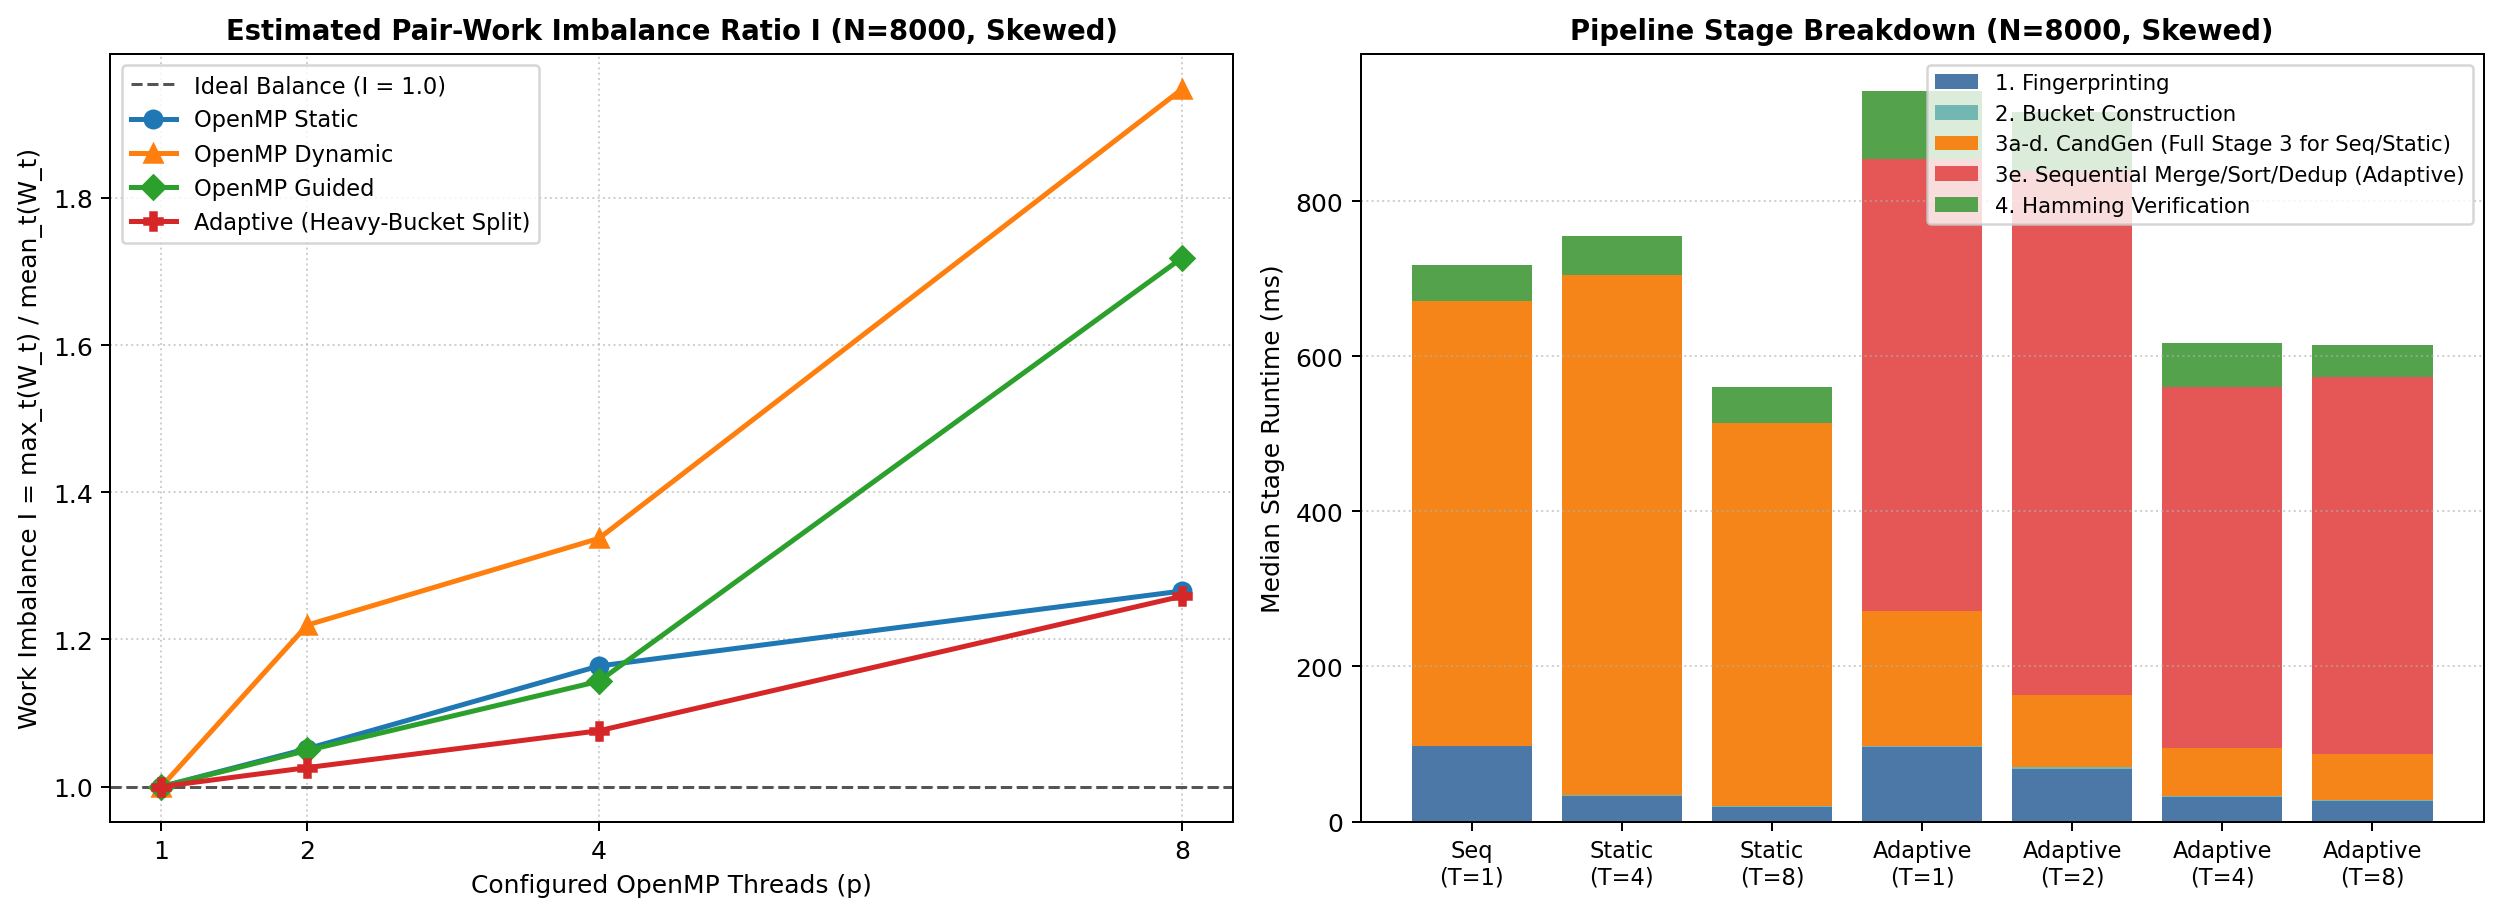
\includegraphics[width=0.92\textwidth]{results/work_imbalance_and_stages.png}
\end{center}
\vspace{-0.35cm}
\fcolorbox{warnorange}{warnbg}{%
    \parbox{0.98\textwidth}{\footnotesize
        \textbf{\color{warnorange}Key Findings --- Work Imbalance \& Stage Bottleneck Analysis ($N=8,000$ Skewed):}
        \begin{itemize}[leftmargin=1.3em, topsep=0.08em, itemsep=0.1em]
            \item \textbf{Thread Load Balance (Left):} \texttt{Adaptive} heavy-bucket splitting maintains the lowest pair-work imbalance across threads ($I = 1.026$ at $T=2$, $1.076$ at $T=4$, and $1.259$ at $T=8$), whereas whole-bucket \texttt{Dynamic} ($I = 1.948$) and \texttt{Guided} ($I = 1.719$) degrade due to tail stragglers.
            \item \textbf{Amdahl's Law Serial Bottleneck (Right):} While parallel fingerprinting (\texttt{Stage 1}) scales by $3.74\times$ and heavy-chunk processing (\texttt{Stage 3d}) scales by $3.04\times$ ($166.95\text{ ms} \to 54.97\text{ ms}$), initial serial candidate merging (\texttt{Stage 3e}, red bar) consumed $\sim 75\%$ of runtime---directly motivating our Phase 9 parallel range-partitioned merge ($-63.2\%$) and Phase 10 SWAR suppression ($-49.6\%$).
        \end{itemize}
    }%
}

\vspace{0.15cm}
\begin{center}
    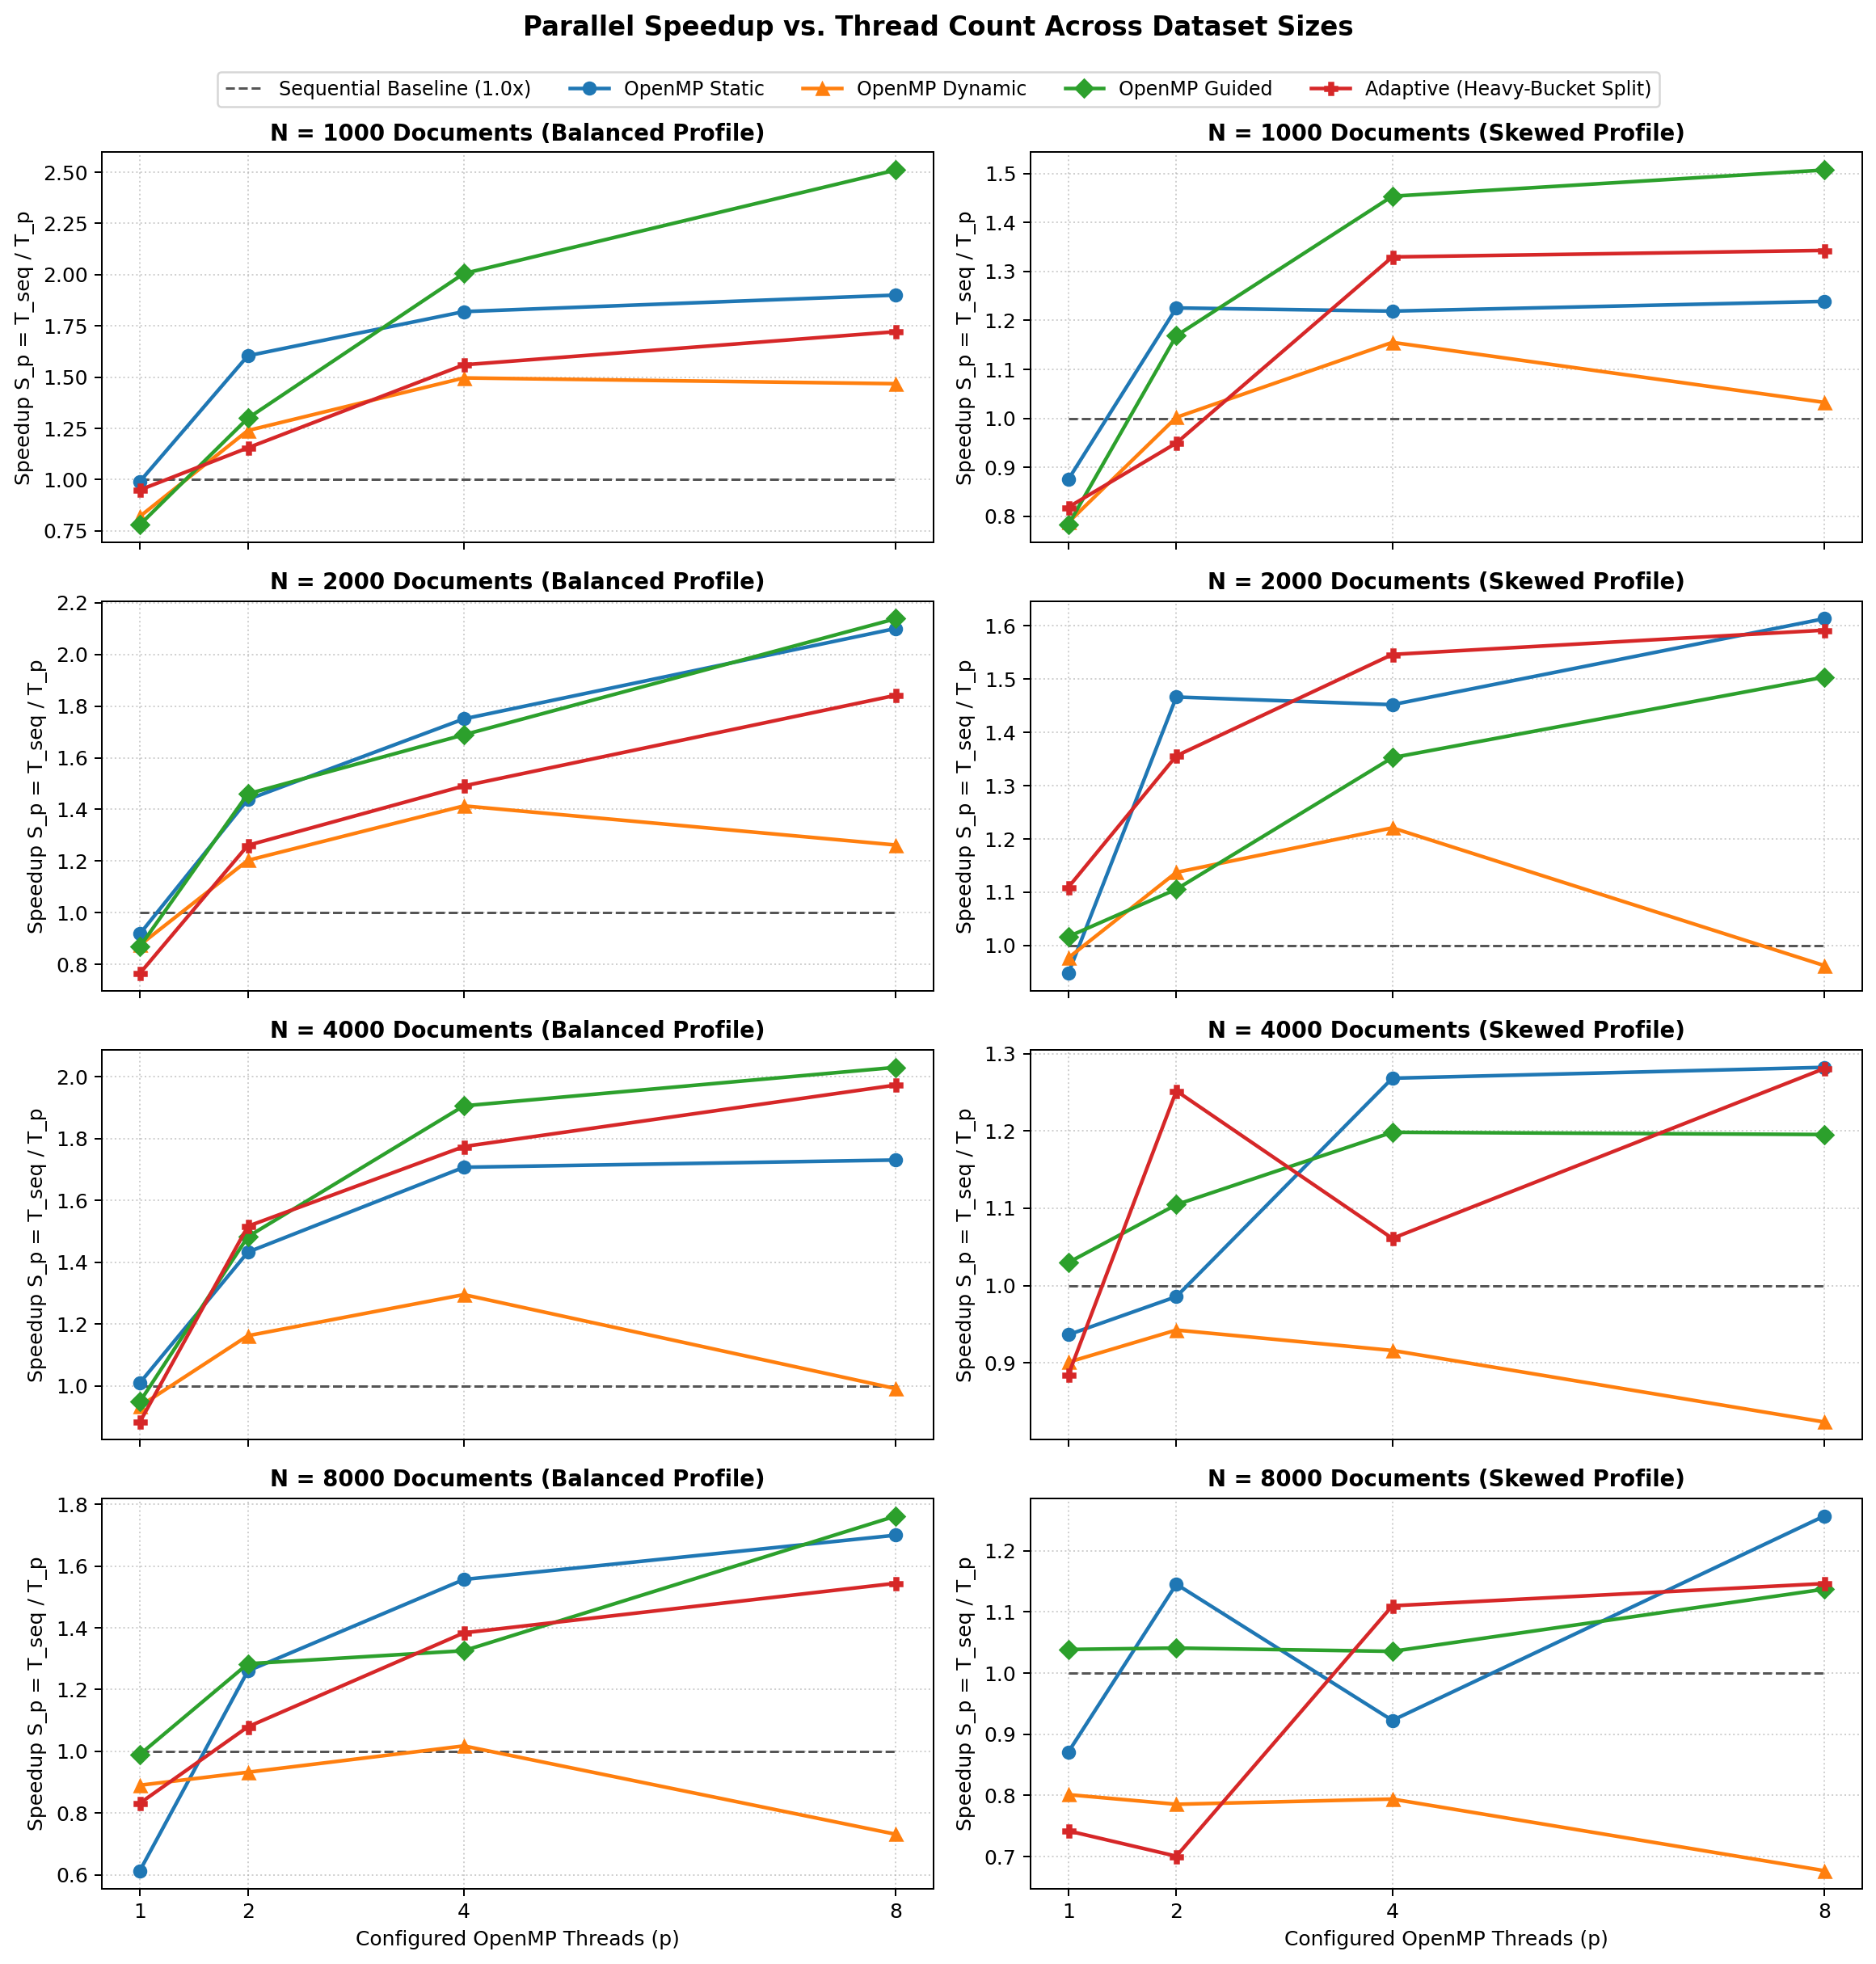
\includegraphics[width=0.63\textwidth]{results/speedup_vs_threads.png}
\end{center}
\vspace{-0.35cm}
\fcolorbox{accentblue}{codebg}{%
    \parbox{0.98\textwidth}{\footnotesize
        \textbf{\color{primaryblue}Key Findings --- Cross-Dataset Parallel Speedup ($N = 1,000$ to $8,000$):}
        \begin{enumerate}[leftmargin=1.4em, topsep=0.08em, itemsep=0.1em]
            \item \textbf{8-Band Structural Symmetry in \texttt{Static}:} Because each 64-bit fingerprint is partitioned into 8 disjoint bands, a dominant duplicate group creates 8 equally sized heavy buckets (one per band $0\dots 7$). Dividing 2,048 buckets into $p \in \{2,4,8\}$ contiguous blocks gives each thread $8/p$ bands and an equal share of the 8 heavy buckets.
            \item \textbf{Stage 4 Queue Contention in \texttt{Dynamic}:} Fixed \texttt{Dynamic} scheduling dispatches $2.73\text{M}$ fine-grained Hamming checks individually through OpenMP's atomic queue, inflating Stage 4 from $36.7\text{ ms}$ to $438.8\text{ ms}$ at $T=8$. \texttt{Adaptive} avoids this by using \texttt{Static} scheduling for uniform-cost Stages 1 and 4 ($40.0\text{ ms}$).
            \item \textbf{Full Thread Utilization:} On $N=1,000$ and $N=2,000$, \texttt{Guided} and \texttt{Dynamic} leave 1--2 threads idle (\texttt{6/8} or \texttt{7/8} participating threads), whereas \texttt{Adaptive} utilizes \textbf{8/8 threads} across all configurations.
        \end{enumerate}
    }%
}

\end{document}
